\documentclass[10pt,twocolumn,letterpaper]{article}

\usepackage{cvpr}
\usepackage{times}
\usepackage{epsfig}
\usepackage{graphicx}
\usepackage{amsmath}
\usepackage{amssymb}
\usepackage{comment}

% Include other packages here, before hyperref.
\usepackage[dvipsnames,table]{xcolor}
\usepackage{color}

% If you comment hyperref and then uncomment it, you should delete
% egpaper.aux before re-running latex.  (Or just hit 'q' on the first latex
% run, let it finish, and you should be clear).
\usepackage[breaklinks=true,bookmarks=false]{hyperref}

% Setup hyperref
\hypersetup{
  colorlinks=true,
  linkcolor=NavyBlue,
  filecolor=magenta,
  urlcolor=cyan,
  pdftitle={Billys: The Bills Classifier},
  bookmarks=true,
}

% *** Custom commands

\newcommand\codeinline[1]{\texttt{#1}}  % alternatives: \mintinline{bash}{#1} or \mintinline{c++}{#1} or \textit{#1}

% *** Config

\cvprfinalcopy % *** Uncomment this line for the final submission

\def\cvprPaperID{****} % *** Enter the CVPR Paper ID here
\def\httilde{\mbox{\tt\raisebox{-.5ex}{\symbol{126}}}}

% Pages are numbered in submission mode, and unnumbered in camera-ready
%\ifcvprfinal\pagestyle{empty}\fi
\setcounter{page}{1}
\begin{document}

%%%%%%%%% TITLE
\title{Billys: The Bills Classifier}

\author{Bryan Lucchetta\\
{\small University of Padua}\\
{\tt\small bryan.lucchetta@studenti.unipd.it}
% For a paper whose authors are all at the same institution,
% omit the following lines up until the closing ``}''.
% Additional authors and addresses can be added with ``\and'',
% just like the second author.
% To save space, use either the email address or home page, not both
\and
Luca Parolari\\
{\small University of Padua}\\
{\tt\small luca.parolari@studenti.unipd.it}
}

\maketitle
%\thispagestyle{empty}

%%%%%%%%% ABSTRACT

\begin{abstract}
Everyone, sooner or later, has to face the messy world of bills. Every
month we get four/five or even more bills, coming from different
providers and about different expenses, with the duty to keep them
safe and easily available in case of need. This task, even if quite
easy, can be very boring for humans. Why don't let that a computer do
it! The main task of our application is, indeed, to put in order this
messy world.  In this paper we present our solution to this
problem. The solution is composed by simple steps, each of them solve
a different task like image dewarping, contrast/illumination
augmentation, textual feature extraction, classification. These simple
steps are then combined in a pipeline which manage the whole process.
\end{abstract}

%%%%%%%%% BODY TEXT

\section{Introduction}

The purpose of our work is to classify bills into some arbitrarily
defined categories (a.k.a., target names or classes), that can
fit almost every bill categories. This targets should help the user to
better handle and organize bills for archiviation. We defined five
classes: \emph{Water}, \emph{Electricity}, \emph{Gas}, \emph{Trash and
  Recycling} and \emph{Telephone and Cable}. For treatability we
assigned to each class an integer from $0$ to $4$,
respectively. Bills are the very foundamental component of the whole
application. A bill, or an invoice, is a commercial document issued by
a seller to a buyer, relating to a sale transaction and indicating the
products, quantities, and agreed prices for products or services the
seller had provided the buyer. In pratical terms, for us, a bill can
be a pdf file or an image (even a camera taken image) to process.

In the following sections we present our work and we face the problems
described above. We start from related works in Section
\ref{sec:related-work}, where we discuss about our starting
point. Then, in Section \ref{sec:dataset}, we present our dataset and
some information about the context of the data we used. After that, in
Section \ref{sec:proposed-method}, we show adopted solutions and
describe smart ideas we used in order to solve the core problem. We
then explore the pipeline and all its components in order to present
full details of what we have done. In Section \ref{sec:experiments},
we also show experiments and fails we have done before getting nice
results. We conclude then with future works and possible enhancements
that for concreteness we excluded from this presentation and we wrap
up with some considerations about the work in Section
\ref{sec:future-works} and \ref{sec:conclusion}, respectively.

\section{Related Work}
\label{sec:related-work}

During our researches, we did not found works that perform this
particular task. However, we found interesting works about different
aspect that we had to face when developing this work.  First of all,
we take into account the image dewarping and feature extraction
problem, that were previously treated in \cite{Korber18} and
\cite{AbbasHussain17}.  Secondly, we had to perform the optical
character recognition from images. In order to do that we relied on
Tesseract, described in \cite{Smith07}, which is a popular open-source
OCR tool developed by Google. Concrete Tesseract usage is shown in
\cite{Benabderrazak20} and \cite{ZelicSable20}, that deal with Python
and Tesseract. The last major step that we had to take into account
was the classification phase, which could be performed by a Naive
Bayes Classifier like the one shown in \cite{ScikitTextDataTutorial}.

\section{Dataset}
\label{sec:dataset}

When dealing with machine learning applications, data are a
foundamental aspect to keep in mind: no data, no party. In fact, in
order to get quite accurate results, a lot of data are needed. For our
application, public domain datasets are very rare, mostly because the
sensible data contained inside each document. For this reason, before
starting with the ``low level'' application we had to collect the
data.

We collected two different dataset that we used to satify our needs
and testing our application during its stages. This two dataset are
described below.

\paragraph{Main Dataset}
\label{par:main-dataset}

The \emph{main dataset} is the first dataset we collected. It is
composed by nearly one thousand bills, where the majority of them are
camera taken photos, while a small part of them are pdfs (either
scanned or the original file).

We tried to keep images with no perspecitive distorsion or other
effects and to exclude the background as much as possibile, because
these corrections are made in a previous pipeline steps. See the full
pipeline in Figure \ref{fig:pipeline}.  In this way we could use the
assumption that documents are already dewarped and we could train the
classifier without being influnced by the preprocessing steps. Even if
we tried to keep the illuminance as good as possible, we included in
the preprocessing phase the brightness enhancing.

While the dataset could be a nice starting point, it has one big
problem: documents do not variate so much. In fact,
\begin{itemize}
  \item documents come from a small number of people, so headers are
    really similar from one document to another;
  \item providers are almost the same, because bills were collected
    from the same local zone;
  \item classes are umbalanced, because some type of bills are less
    frequent than others.
\end{itemize}

The Table \ref{table:main-dataset} shows the composition of our
dataset.

\bgroup
\def\arraystretch{1.5}%
\begin{table}[!h]
  \begin{center}
    \begin{tabular}{p{1.5cm} p{1.2cm} p{1.2cm} p{3cm}}
      \hline
      Categories                 & Number of Documents & Number of Providers & Providers                                                             \\ \hline
      \emph{Telephone and Cable} & 403                 & 9                   & Vodafone, Wind, Tre, Wind Tre, Telecom, TIM, Tele 2, Fastweb, Teletu  \\
      \emph{Electricity}         & 276                 & 6                   & Green Network, Servizio Elettrico Nazionale, Etra, Enel, Edison, Hera \\
      \emph{Gas}                 & 202                 & 4                   & Sorgenia, Ascotrade, Etra Energia, Hera                               \\
      \emph{Water}               & 123                 & 3                   & Etra, Alto Trevigiano Servizi, Hera                                   \\
      \emph{Garbage}             & 45                  & 1                   & Savno                                                                 \\ \hline
      \textbf{Total}             & 1048                & 19                  &                                                                       \\ \hline
    \end{tabular}
  \end{center}
  \label{table:main-dataset}
  \caption{Main dataset composition.}
\end{table}
\egroup

\paragraph{Warped Dataset}
\label{par:warped-dataset}

The \emph{warped dataset} is instead the second dataset we collected
and it consists of nearly one hundred and fifty camera taken photos of
our home bills, as in the main dataset, but in this case they are
taken with perspective distorsion, rotation and with parts of the
background. With this dataset we are able to test the full
pipeline. The results obtained with this dataset and with the full
pipeline are reported in Subsection
\ref{subsec:naive-bayes-classifier}.

\section{Proposed Method}
\label{sec:proposed-method}

The task itself is very complex and can lead to a messy and
unmantainable solution. For this reason we develop a robust and well
structured pipeline with the aim to face some of the main problems,
described below.

\begin{itemize}
  \item \textbf{Image dewarping}: camera taken image are usually not
    directly processable by an optical recognition tool. In order to
    perform the OCR we have to preprocess the image and rotate, resize
    and strech it.
  \item \textbf{Contrast/illumination correction}: also the
    illumination/contrast of an image can be a nasty problem for an
    OCR tool, as it needs a clear distinction between written text and
    other stuff in the image.
  \item \textbf{Optical Character Recognition}: the OCR can be a very delicate
    point, as the application performances depends on how the OCR
    extracts data from images.
  \item \textbf{Text preprocessing}: a huge amout of details can be extracted
    from the OCR, but surely not all of them are relevant for
    application's purposes. We need to disregard them for good results.
  \item \textbf{Feature classification}: at the end, our need is to classify
    the given object. This is a complex task as document data can be
    very different and very similar at the same time.
\end{itemize}

To resolve all these problems we prososed the pipeline reported in
Figure \ref{fig:pipeline}.

We choose to use an Optical Character Recognition instead of a
Convolutional Neural Network because the classification mostly depends
on the content of the document, while the global image shape does not
matter so much.  Another reason for this choice, is that a CNN needs a
lot of examples to be trained on: collecting such a dataset would have
been a big problem Once we have chosen to include an OCR tool, all the
rest of the pipeline is built considering the major drawback known for
OCRs (page dewarping and brightness enhancing).

\begin{figure*}[!ht]
  \centering
  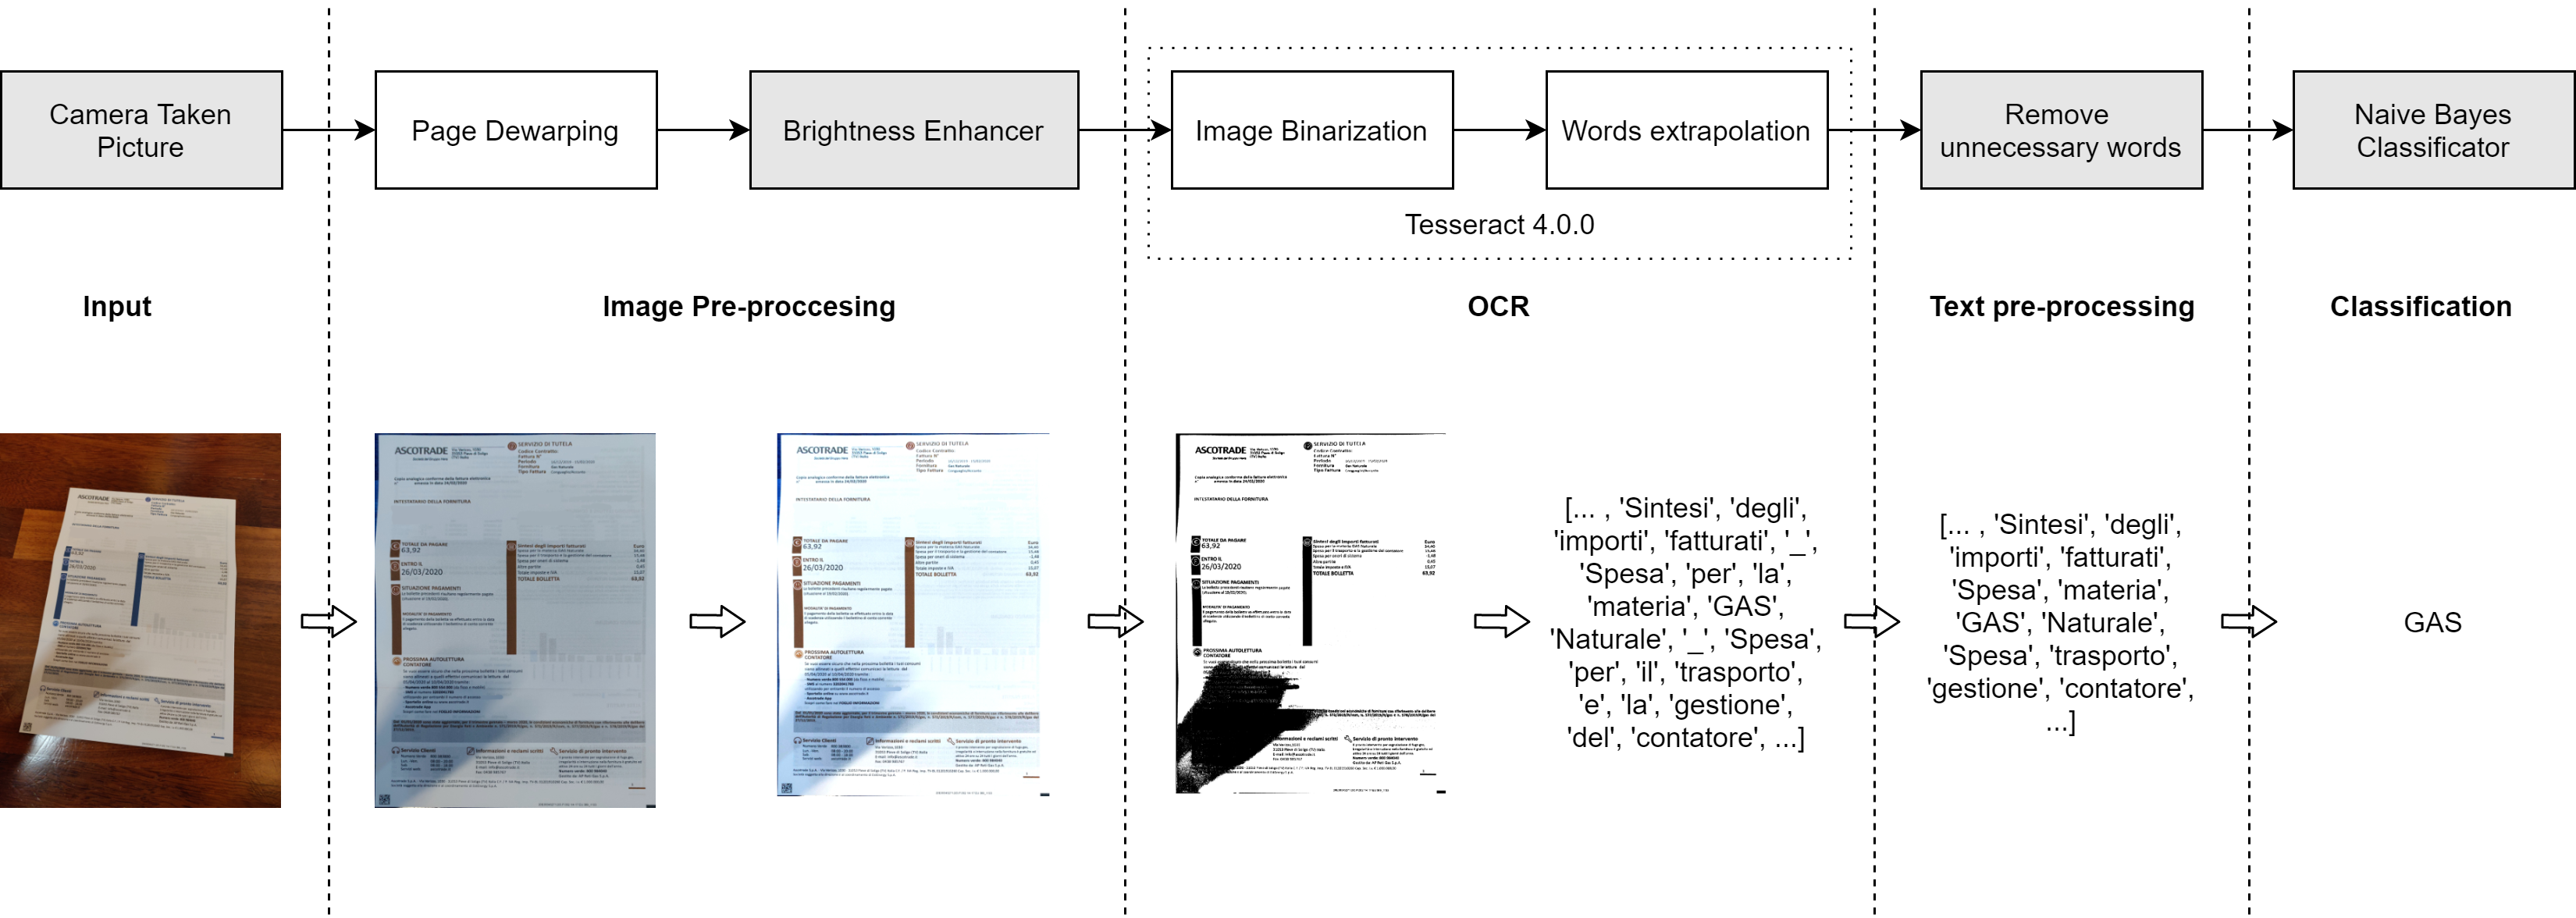
\includegraphics[width=1.0\textwidth]{images/pipeline.png}
  \caption{Our pipeline}
  \label{fig:pipeline}
\end{figure*}

\subsection{Image Preprocessing}

The image preprocessing is a crucial point in our application. Its
main responsability is to adjust all the aspects of a mobile camera
taken photo. This includes enhancing brightness and contrast,
dewarping, skew correction and others.

The first in order to recover a nice image is the dewarp. For this
task we started from the work done in \cite{Korber18} wich uses an
Xception Neural Network (see \cite{Xception}) to perform this task,
with appreciable results according to the article. In Subsection
\ref{subsec:xception-nn-architecture} we describe the Xception Neural
Network architecture while the Figure \ref{fig:xception-architecture}
pictorially shows it.

The second step is contrast/illumination adjustment. A good
illumination of an image is crucial for a good OCR result. Refer to
the Section \ref{subsec:camera-taken-illuminance-quality} for further
details.

\subsubsection{The Xception Neural Network}
\label{subsec:xception-nn-architecture}

The dewarping phase is completly based on the work done in
\cite{Korber18}. Accordingly to the author, the recovery of the
homography of a mobile camera taken photos of a document is delegated
to a Xception Neural Network. The paper \cite{Xception} describes this
architecture ans shows how it heavily relies on prior efforts in the
Inception architecture which first demonstrated the advantages of
factoring the convolutions into multiple branches operating
successively on channels and then on space. Also, this architecture is
entirely based upon the Residual Connections and Depthwise separable
convolutions. This aspects are treated in \cite{Sahoo17} and
\cite{Wang18}, respectively.

The used Xception Neural Network is trained over $1.5$ million
synthetic images. It uses the \emph{Adam} optimization method in
combination with the \emph{L1-loss} to predict the four corner points
of the distorted image. Then given these corners, the homography
matrix $H$ is computed using a \emph{Direct Linear Transform} (DLT)
algorithm. The network is made of thirtysix convolution layers and
more than twenty million trainable parameter.

\begin{figure}[!ht]
  \centering
  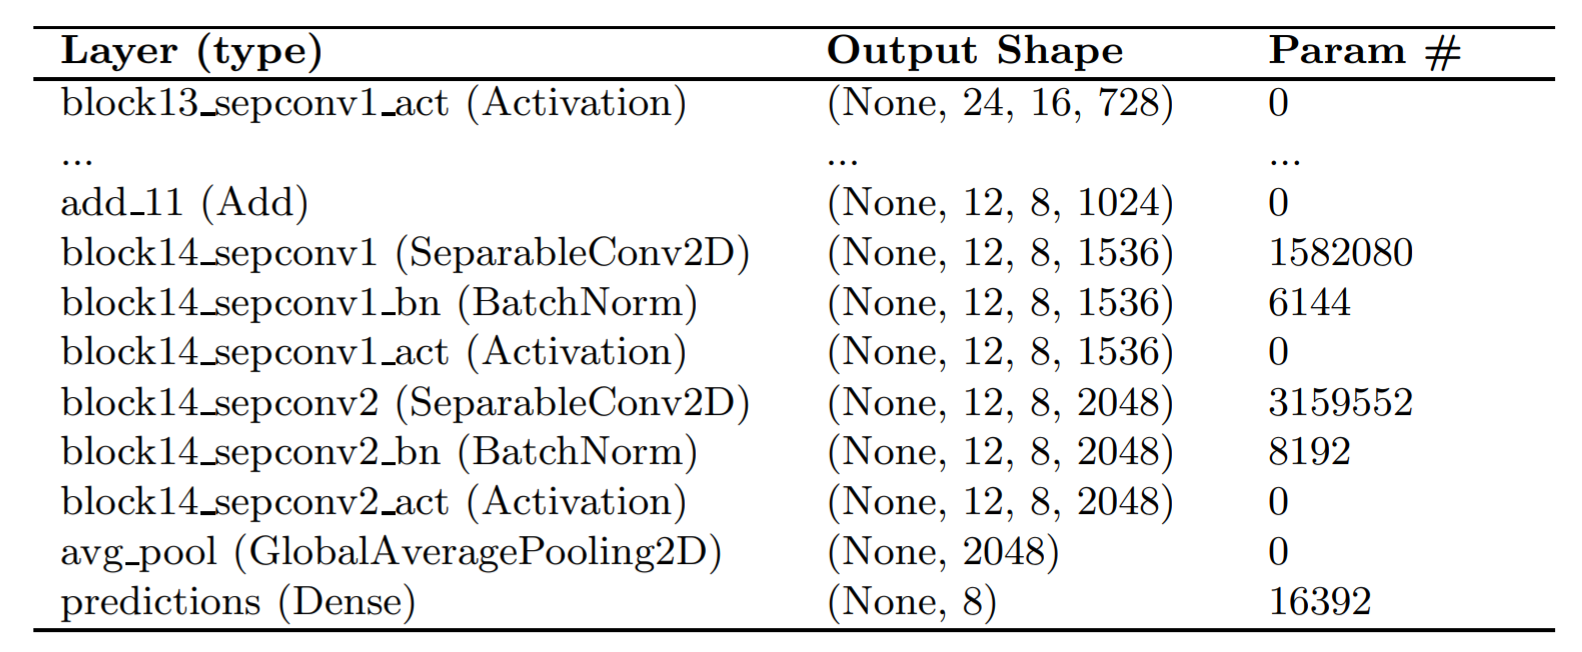
\includegraphics[width=0.48\textwidth]{images/xception-architecture.png}
  \caption{The Xception architecture used in this work}
  \label{fig:xception-architecture}
\end{figure}

We empirically noticed a sort of bug in the network: it do not dewarp
images with extreme conditions of contrast/illumination, but this is
not really a problem as the exepriment in Subsection
\ref{subse:dewarping-or-not} shows.

\subsection{Optical Character Recognition}

The OCR task can be a very complex part of the pipeline. So, instead
of focusing on already developed tools we decided to delegate the OCR
task to Tesseract. Tesseract is an open-source, optical character
recognition tool developed at Google and it source code is freely
available on GitHub under the Apache License, Version 2.0.

Tesseract works out-of-the-box with sveral languages, included
italian. So, as the good realiability of Tesseract we decided to used
it as a black-box and focus on more delicated tasks.

\subsection{Text Preprocessing}

The text preprocessing phase is an important task that may occur
immediatly after the textual features extraction from images. The aim
of this task is mainly to preprocess the plain text coming from images
in order to remove non-relevant features: pratically, it transforms the
text into a more digestible form so that machine learning algorithms
can perform better.

The implementation of this step follows some very simple ideas for
text preprocessing. Indeed, we just normalize the text into its base
form. The inner pipeline for this phase is composed by atomic steps,
described below. Note that for this task, the execution order of some
steps really matters, so we ordered them for better performances.

\begin{enumerate}
  \item \textbf{To lowercase}: the first step for the text normalization is to
    remove differences from uppercase and lowercase letters.
  \item \textbf{Remove accented characters}: accented chars, specially in
    italian, are often used. However for our task they are not relevant
    and the OCR may also miss them, so we decided to exclude them from
    the principle and to represent words with their non accented
    versions.
  \item \textbf{Remove punctuation}: also the punctuaction do not really
    matters, and indeed cannot say anything on the class of the bill
    that we are considering, so we decided to remove them.
  \item \textbf{Remove numbers}: bills can be full of numbers and we
    can find them under many forms, as, for example, dates,
    identifiers, furniture comsumption, and so on. However, also
    numbers cannot say anything about the bill class, so they were
    removed and replaced with the keyword \codeinline{<num>}, which
    instead can be more informative as when vectorized in bag of words
    its numerosity is associated with the the number of numbers in a
    bill. For this case, we decied to do not completely remove the
    information but to keep only its condensed version.
  \item \textbf{Remove stopwords}: in order to obtain the most informative
    textual representation of a bill we had to remove also
    insignificat words like stopwords. Stopwords are words that can be
    used frequently in phrases, so in the context of representing the
    bill class, an article isn't informative. Stopwords are remove
    with the help of the \emph{Natural Language Toolkit}, available as
    a python package: \emph{nltk}. NLTK provieds a collection of
    stopwords, that can be easily downloaded with
    \codeinline{nltk.download('stopwords')}, and then, with
    \codeinline{nltk.corpus.stopwords.words('italian')} we can obtain the
    localized version of the stopwords and perform the removal.
  \item \textbf{Remove shortwords}: By means of experiments we discovered that
    the OCR phase, under certain (bad) conditions, returns parts of
    words, usually very smaller. We empirically found that by removing
    this ``shortwords'', we could improve performances.
  \item \textbf{Lemmatize}: lemmatisation (or lemmatization) in linguistics is
    the process of grouping together the inflected forms of a word so
    they can be analysed as a single item, identified by the word's
    lemma, or dictionary form.\footnote{\href{
        https://en.wikipedia.org/wiki/Lemmatisation}{
        https://en.wikipedia.org/wiki/Lemmatisation}} With
    this step, indeed, we tried to group words together in order to
    simplify the classification phase. However, we noticed that this
    step do not improve the performance and it can also produce worst
    results as it tries to group wrong words retrieved from the OCR.
  \item \textbf{Tokenize}: at the end of the preprocessing we create a list of
    words (Tokenization), that can be easily represented by in a
    vectorized form.
\end{enumerate}

\subsection{Features Classification}
\label{subsec:classification}

The features classification is itself a core step, needed for the real
bills classification. Indeed, the pipeline steps before the features
classification can be viewed as a giant image preprocessing step, with
the goal to preprare a nice subset of features to be used in the
classifier.

Regardless of the chosen implementation for a classifier, textual
features need a transformation in order to be handled: we need to
transform text into numerical feature vectors. In order to do this, we
can use the \emph{bag of words} technique, that is based on the
following strategy:

\begin{itemize}
  \item Assign a fixed integer id to each word occurring in any
    document of the training set (for instance by building a
    dictionary from words to integer indices).
  \item For each document $i$, count the number of occurrences of each
    word $w$ and store it in $X[i, j]$ as the value of feature $j$,
    where $j$ is the index of word $w$ in the dictionary.
\end{itemize}

Once we have the bag of words we can analyze words occurency in order
to extract frequencies. We cannot rely on occurrencies because longer
documents will have higher average count values than shorter
documents, even though they might talk about the same topics. To avoid
these potential discrepancies it suffices to divide the number of
occurrences of each word in a document by the total number of words in
the document: these new features are called \emph{Term
  Frequencies}. Another refinement on top of \emph{tf} is to downscale
weights for words that occur in many documents in the corpus and are
therefore less informative than those that occur only in a smaller
portion of the corpus. This downscaling is called \emph{Term Frequency
  times Inverse Document Frequency} (\emph{tf-idf} for brevity).

Now, we are ready to train the classifier in order to predict a bill
category. For completing this task we proposed two strategies: a
``deterministic'' classifier and a Naive Bayes classifier. The
deterministic classifier is based on the simple idea that each
document category has a small subset of words that are very relevant
for the classification. Indeed, we have arbitrary defined the
vocabulary that specifies what words we expect to find in a document
based on its category. Then, the classifier applies a simple
algorithm, which works as follows:

\begin{itemize}
  \item Compute the frequency of each word in a given bill;
  \item For each word, if it is a relevant word\footnote{A word $w$ is
    a relevant word if it is contained in some keyword $kw$ and the
    longest common subsequence between $w$ and $kw$ is at least
    $\mathrm{len}(kw) - 1$.}, sum its contribution to the aggregate
    sum of the category of that word;
  \item Return the class which has more contributes.
\end{itemize}

The Figure \ref{table:determnistic-classifier-dict} shows an example
of the vocabulary (italian version) we used to perform bills
classification, how we can see, it is very small and effective.  On
the contrary, one could think to automatically generate the
vocabulary: this could be a valid option! See the Section
\ref{sec:future-works}.

Obviously the deterministic classifier is not the only way to perform
the classification task, in fact, we experimented also a Naive Bayes
Classifier. See Subsection \ref{subsec:naive-bayes-classifier}.

\bgroup
\def\arraystretch{1.3}%
\begin{table}[!h]
  \begin{center}
    \begin{tabular}{p{2cm} p{5cm}}
      \hline
      Class                 & Keywords                                                                                                                                                    \\ \hline
      Water                 & acqua, idrico, depurazione, fognatura, trevigiano                                                                                                           \\
      Garbage and Recycling & spazzatura, immondizia, riciclato, riciclo, rifiuti, rifiuto, savno, igiene, ambientale                                                                     \\
      Gas                   & gas, naturale                                                                                                                                               \\
      Electricity           & luce, energia, tensione, potenza, chilowatt, elettricita, elettrico, elettrica, green, enel, edison                                                         \\
      Telephone and Cable   & telefonia, telefonate, telefonico, chiamate, canoni, fibra, internet, ricaricabile, ricarica, cellulare, navigazione, telecom, vodafone, tim, fastweb, wind \\ \hline
    \end{tabular}
  \end{center}
  \label{table:determnistic-classifier-dict}
  \caption{A vocabulary for the deterministic classifier.}
\end{table}
\egroup

\section{Experiments}
\label{sec:experiments}

\subsection{Dewarping or not?}
\label{subse:dewarping-or-not}

Camera taken images can present lot of irregularities like small
rotation, perspective distortion and so on. However, even if this
small defects are not a problem for a human, they can be for an
automatic tool. In order to test the effectiveness of the dewarping
phase, we proccessed the same images two times: the first without
dewarping and the second with the dewarping. The results were quite
surprising. Indeed, watching at the ``boxed'' image we could notice
that the OCR extracted many more words from the image without
dewarping than the one with, but the plain output was not so precise
and contained a lot of blank characters. An example is shown at Figure
\ref{dewarping-experiment}. In that picture we can see two ``boxed''
images, where the green boxes represents OCR detected words. The left
image is not dewarped while the right is. From the left image we could
extract $708$ words, while for the right one only $491$. However, the
text extracted from the left image contains a lot of black characters
and the precision of read words is low, while the right image has a
very high precision and fewer blank characters.

\begin{figure}[b]
  \centering
  \includegraphics[width=0.48\textwidth]{images/dewarping-experiment.png}
  \caption{Difference with and without dewarping phase text extraction}
  \label{dewarping-experiment}
\end{figure}

Moreover we tried to do the classification of the photos contained in
the warped dataset and with a Naive Bayes Classificator trained on the
main dataset without dewarping the photos. In this case we obtained an
accuracy of $64\%$ instead of $95\%$ obtained with the same dataset but
with the dewarping phase enabled.

This experiment empirically confirms that the dewarping phase is an
important task when dealing with OCR tools and in that specific task
it has improved the perfomance by $30\%$.

\subsection{Camera Taken Illuminance Quality}
\label{subsec:camera-taken-illuminance-quality}

A good illumination on images is often the key for a good
OCR. Tesseract, the designated tool for OCR, already preprocess images
internally, and it tries to binarize it for the text extraction phase.
The problem of this preprocessing step arises when the taken photos
have a bad illumination or there are shadows. An example of this
behaviour is shown in the Figure
\ref{bright-constrast-experiment}. The first part of the example shows
as the binarization acts on bad illuminated images.  Instead, if we
increase brightness we can see that the binarization is better as it
do not throw away most of the text. With this improvemets also the
text extraction performances increase.

\begin{figure}[!ht]
  \centering
  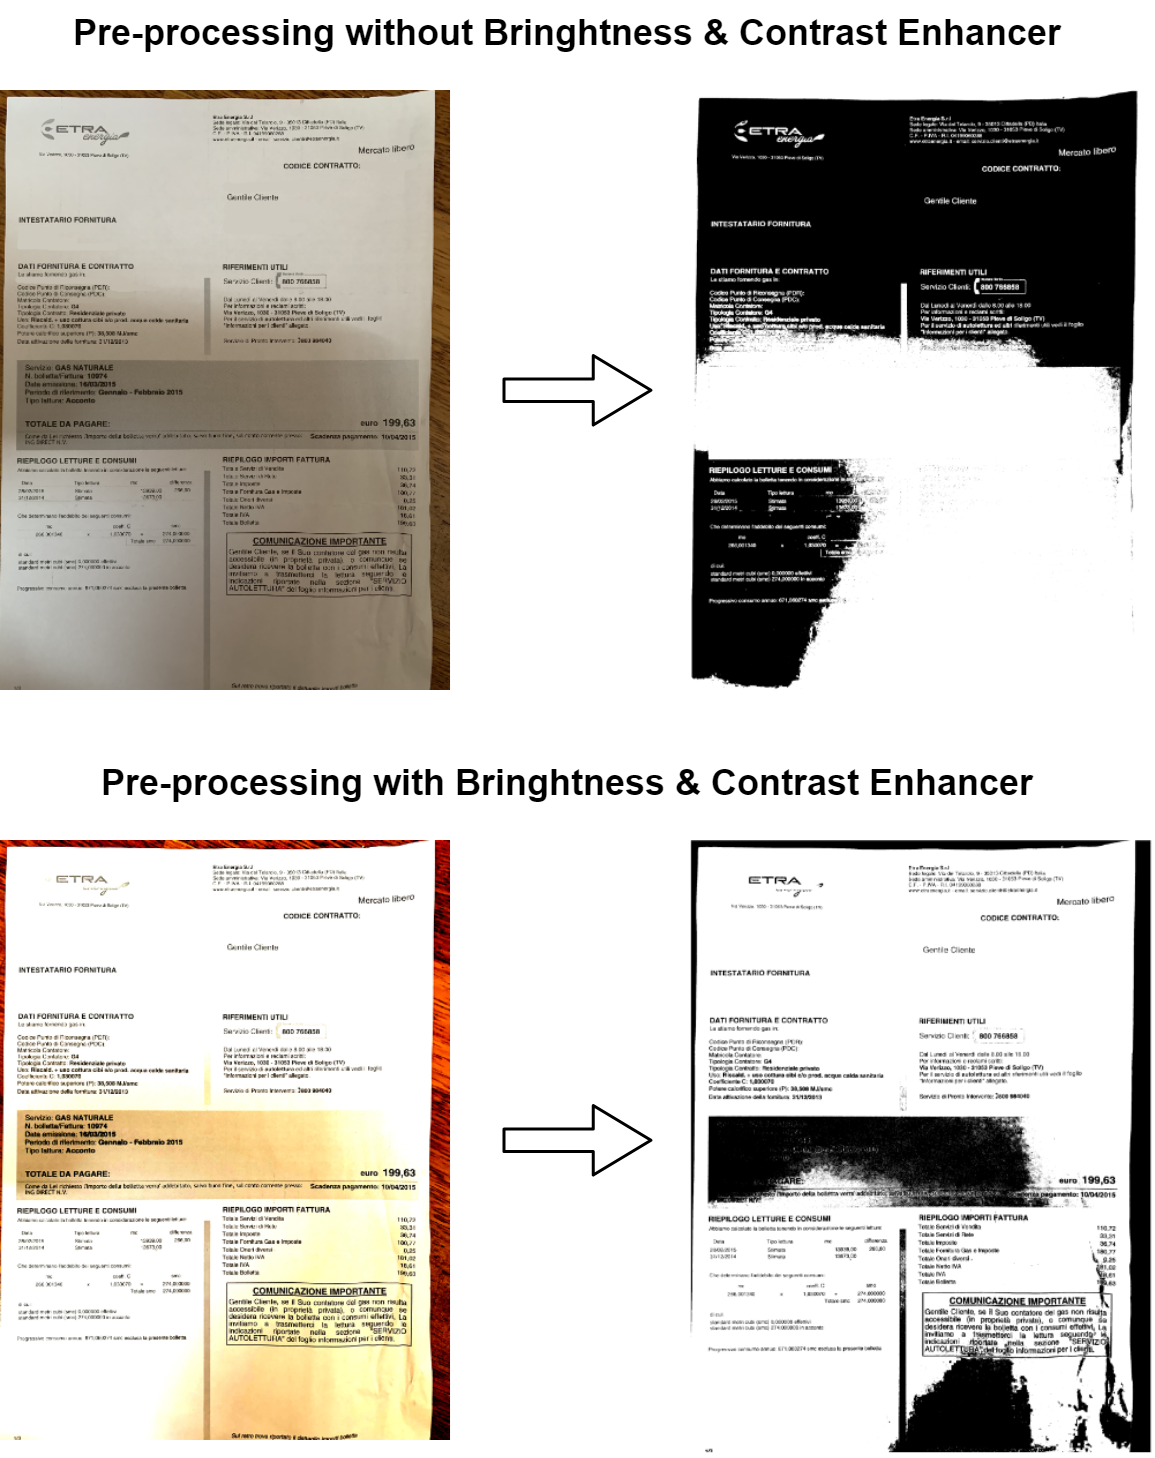
\includegraphics[width=0.4\textwidth]{images/bright-contrast-experiment.png}
  \caption{Difference with and without Brightness Enhancer}
  \label{bright-constrast-experiment}
\end{figure}

After theese consideration we introduced the \emph{brightness
  enhancing} step in our pipeline for all images, excluding scanned
documents and pdfs.

We could empirically confirm those improvements with some
tests. Theese tests were conduced on the water class (wich was the
more problematic in terms of image illuminance): without brightness
enhancing the accuracy was $94\%$, while with it accuracy was $99\%$.

Many more improvements can be obtained tweaking illuminance an
contrast augmentation. Also, another improvement, as reported in
Section \ref{sec:future-works}, could be a system that automatically
set the illumination gain for each image.

\subsection{Naive Bayes Classifier}
\label{subsec:naive-bayes-classifier}

The deterministic classification strategy proposed in Section
\ref{subsec:classification} is not the only feasible way. There are
many machine learning algorithms applicable with text classification:
one over the other is Naive Bayes.

The Naive Bayes classifier, unlike the deterministic classifier, comes
from the family of simple probabilistic classifiers based on applying
Bayes' theorem with strong (naive) independence assumptions between
the features. Indeed, it calculates the probability of a certain word
to be seen in a document and it uses that probability in
classification phase for predicting the document class. For our task
we need the Multinomial Naive Bayes classifier, as we have to predict
multiple classes, not only $0$ or $1$.

Due to the definition of our problem, this type of classifier
is probabily an overkill: it bases the predicted target on all the
text provided to the classifier. Under our domain, documents are very
likely to be similar for most of their parts and we have only few
interesting words for each document that differs. Also, bills contains
huge amount of non-relevant data for our application like marketing
banners, disclaimers, formal opening of letters, and so on. Another
problem we had, as described in Section \ref{sec:dataset}, is the
problem of the headers: we can have two bills about different
categories with same header (same user data), or bills about same
category with different headers (different user data).

Anyway, as Naive Bayes usually performs very well we tried an
implementation tuned with a grid search strategy. Then we evaluated
its model performances on another dataset composed by unseen bills
with different headers and providers, and we discovered that it
performs almost the same as the deterministic classifier.  However, we
must underline that this third dataset was composed by very very few
images, so the results are not reliable.

\paragraph{Results}

The Table \ref{table:classifiers-comparison} shows a comparison
between the performance of the main and the warped dataset (described
in Section \ref{sec:dataset}), for the Naive Bayes classifier trained
on our main dataset and the deterministic classifier. In the warped
dateset, we enabled and disabled the dewarping phase to see the
difference in performance with this task.

\begin{table}[!h]
  \begin{center}
    \begin{tabular}{lll}
      \hline
      Classifier              & Accuracy & Support \\ \hline
      \textbf{Main Dataset}                        \\
      \small Without dewarping phase               \\
      \; \; Naive Bayes       & $0.99$   & $1047$  \\
      \; \; Deterministic     & $0.99$   & $1047$  \\ \hline

      \textbf{Warped Dataset} &          &         \\
      \small Without dewarping phase               \\
      \; \; Naive Bayes       & $0.59$   & $129$   \\
      \; \; Deterministic     & $0.40$   & $129$   \\

      \small With dewarping phase                  \\
      \; \; Naive Bayes       & $0.98$   & $129$   \\
      \; \; Deterministic     & $0.88$   & $129$   \\ \hline
    \end{tabular}
  \end{center}
  \label{table:classifiers-comparison}
  \caption{Accuracy comparison between Naive Bayes classifier and
    deterministic classifier.}
\end{table}

As we can see, the dewarping phase really matters. Howevere, as we
have particular dataset without a good variance, we can hypotize that
the two behave in the same way, but Naive Bayes can also recognize non
relevant words and do a good job even with the warped dataset.

\section{Future Works}
\label{sec:future-works}

The task offers a infinite list of related works that can be done in
order to improve results and extends our ideas. We list below some of
possible future works.

\begin{itemize}
  \item Enhanced text preprocessing. Our text preprocessing is not
    sophisticaded, instead it is composed by the necessary steps in
    order to get a decent classifier. An enhance on text preprocessing
    could be the header removal. Under the bills domain, headers are
    composed of extremenly non-relevant data, that could be discarded
    with a vocabulary of names or something similar.
  \item Automatic vocabulary building for deterministic
    classifier. For concreteness, we manually built the vocabulary
    used in the deterministic classifier, instead one could let the
    machine generate it. In fact, our approach has some drawbacks: the
    application tends to be static, but mainly, the vocabulary can
    miss some relevant words. A well configured vocabulary automatic
    building can surely perform better wrt the manual one.
  \item Automatic contrast/illumination gain. Our illumination
    enhancing technique is based on a parameter, namely \emph{gain},
    which is manually setted before the whole pipeline execution and
    is responsible for the contrast/illumination augmentation. An
    interesting improvement could be a system which can decide itself
    how much gain use for the contrast/illuminanche augmentation. In
    fact, we noticed that with the wrong gain values performances can
    be very poor and surely a single value for each sample provided
    is not the best choice.
  \item Enhanced Dewarping. As we shown in the Table
    \ref{table:classifiers-comparison}, a good image dewarp can really
    help in classification. Indeed, another improvement could be a
    fine tuning for the dewarp system. The goal is obtain a network
    which is really good in finding sheet of paper corners and return
    them for the real dewarping. An idea is to train a neural network
    on a relatively huge dataset that contains image where in the
    foreground there is a sheet of paper (even with perspective
    distorsion and rotation) and in the foreground tables
    textures. This would help a lot as the dewarp performs very bad
    when the background has the same color of the document in the
    foreground.
\end{itemize}

\section{Conclusion}
\label{sec:conclusion}

From this experience we can first of all conclude that data are the
real core of nowdays applications, specially for the machine learning
ones: having a good dataset is, we would say, the hardest part of the
whole project, bacause all results depends on the data you have. We
also learned a lot about image preprocessing and feature extraction
from images: the only fact that a simple rotation or perspective
distortion can catastrophically change what features can the OCR
extract, was very desturbing. We spent a lot of time on image
preprocessing as in a concrete context users do not pay much attention
on the way they make photos. Another part where we dedicated lot of
time was the classification part. In fact, that part was one of the
harder because the complexity of the pipeline: a small change on the
contrast preprocessing phase leads to a significant change on the
classification stage.

However, we are really happy with this experience and the obtained
result and we know that the work can still be improved by taking into
account all the ideas and considerations made in this report.

The project is available also on GitHub:
\begin{center}
  \href{https://github.com/lparolari/billys}{https://github.com/lparolari/billys}
\end{center}

{\small
\bibliographystyle{ieee_fullname}
\bibliography{egbib}
}

\end{document}
